% EXISTING SOLUTIONS
% existing solutions

% intro

Three systems will be discussed in this area, each one bearing goals in common
with the multimodal solution idealized here.

ARVIKA is useful in the sense that the biggest project so far in Augmented Reality
domain came up with a working solution to aid in industrial tasks but leaving most
of the regular user interfaces intact -- there's space for improvement here.
Additionally it lacked an authoring tool to provide the end-users the means to
easily setup scenarios.

Speech and Gestures shows a project where the Google Earth \cite{SITE-EARTH} application, a single
user system that allows navigation in a world representation has been adapted to
work in a multi-touch surface with speech recognition.
The adapting work provided feedback about the limitation such software faces 
and a working solution to map most Google Earth actions as speech and gesture counterparts.

Finally Digital Whiteboard is introduced. It provides a solution to a multi-user digital
whiteboard where each user handles a palmtop that serves as both each user's palette and
private composing area, for writing text or preparing drawings.
A technique called pick-and-drop is then explained. It is used to allow a user to insert
the contents of each palmtop to the shared whiteboard.


\subsubsection{ARVIKA, 2003}

ARVIKA \cite{ARVIKA} is a project with sponsoring from the
German Federal Ministry of Education and Research that took place between 1999 and 2003.
It focused on the development of Augmented Reality (AR) technologies to aid in industrial tasks.
The consortium involved several industrial partners, such as Volkswagen, BMW, Siemens and Airbus.

\begin{figure}[!ht]
    \centering
    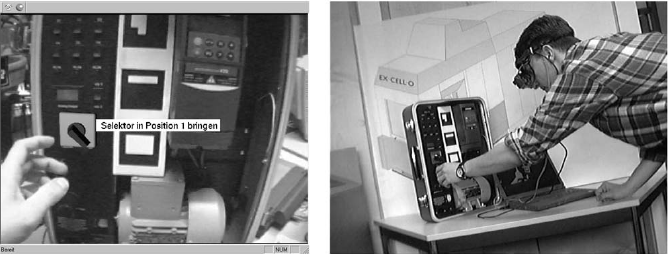
\includegraphics[width=10cm]{gfx/arvika.png}
    \caption{The augmented view seen from the HMD; a user of the ARVIKA system}
    \label{FIG-ARVIKA}
\end{figure}

An expert in the industrial area carried a head mounted display with a camera mounted on it.
The real-time captured video was then interpreted and markers extracted from the image.
The camera's position and orientation was estimated and the head mounted display view was
enriched with virtual objects (see figure \ref{FIG-ARVIKA}, left).

The framework was distributed in the form of an ActiveX plug-in for the Internet Explorer Browser
named ARBrowser.

\paragraph{Discussion}
\label{sec:Discussion}

Weidenhausen et al. \cite{ARVIKA-LESSONS} consider the deployment of the project as an ActiveX component
to be an advantage since it is based on a widespread program (Internet Explorer) and allowed developers
to create task scenarios with JavaScript and HTML.

Although the world's largest research project in the area, ARVIKA focused too
much on the technical problems regarding AR and little effort was spent on the creation of a
suitable user interface. The authors agree that most people judge the usefulness of a technology
mainly by its user interface, therefore this particular topic became work for future project iterations.

ARVIKA was meant to support many industrial scenarios -- development, production and service for several
industrial partners in different domains. Creating a scenario was a time consuming task -- taking several days,
according to Weidenhausen et al. -- and required extensive knowledge in 3D modeling tools and VRML.
No authoring capabilities were therefore given to end-users.
This problem was identified as paramount and an authoring tool was scheduled for development,
supporting generic task creation with parameters controlled by the users.



\subsubsection{Speech and Gestures on a Multi-User Tabletop, 2006}

Tse et al. \cite{SP-GEST-TTOP} developed a multimodal interface on top of Google Earth \cite{SITE-EARTH} to be run
on a multi-touch table. The system allowed multi-user collaboration with touch and voice commands.

The main problems found in adapting Google Earth concern it being a single user program, where only
one action can be done at a time.

In this scenario several users can be oriented differently around the table, so text readability problems arise.
Some user interface components such as the compass were placed at fixed points on the screen, places that
don't make sense on a multi-user scenario.

At 1024 x 768 resolution it was estimated that 42\% of the screen was originally consumed by GUI elements.

Feedback is another important feature. Most Google Earth interactive actions were mapped into gestures, leaving
the most abstract actions to voice commands (see figure \ref{FIG-SP-TABLETOP2}).

Since all users share the same surface turn taking protocol was free floor, leaving the users to regulate
their turns using social protocol.

\begin{figure}[!ht]
    \centering
    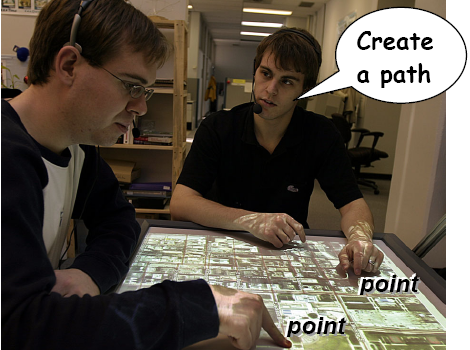
\includegraphics[width=7cm]{gfx/sp-gest-ttop.png}
    \caption{Two users collaborating on a Google Earth tabletop session}
    \label{FIG-SP-TABLETOP}
\end{figure}

\begin{figure}[!ht]
    \centering
    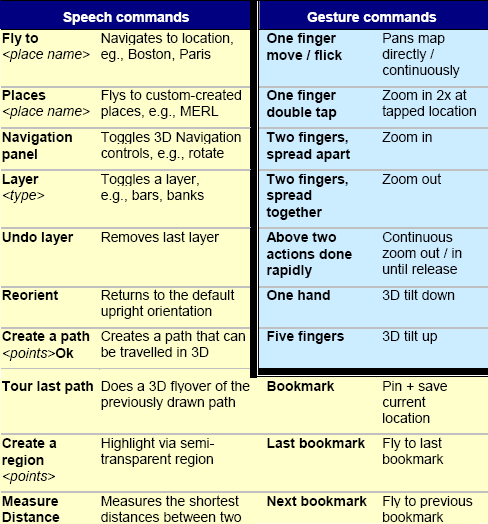
\includegraphics[width=8cm]{gfx/sp-gest-ttop2.png}
    \caption{The suggested speech and gesture interface for Google Earth}
    \label{FIG-SP-TABLETOP2}
\end{figure}

\paragraph{Discussion}
\label{sec:Discussion}

Google Earth is a good example of a navigation system. It provides several functionality
and could support the creation of buildings. This example shows both the need to develop
a better solution for collaborative scenarios and a working multimodal solution mapping
most of its interface.



\subsubsection{Digital Whiteboard, 1998}

Rekimoto \cite{WBOARD} presents a digital whiteboard where each participant is given
a palmtop computer to handle. It works as a tool palette, remote commander, text entry box as
well as a temporary data buffer during whiteboard collaboration interaction.

\begin{figure}[!ht]
	\centering
	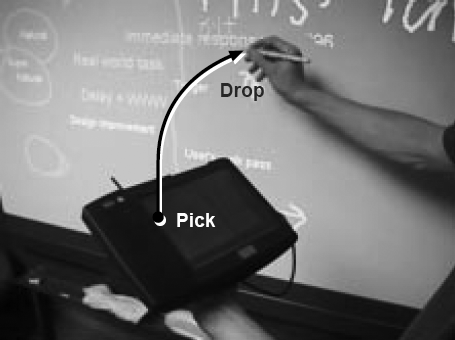
\includegraphics[width=6cm]{gfx/wboard.png}
	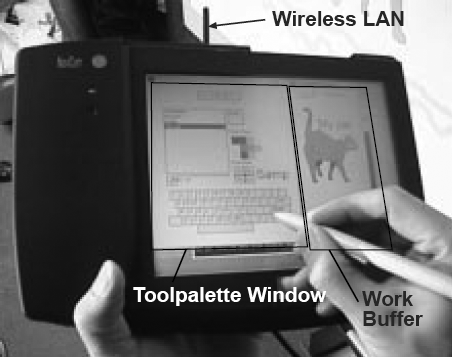
\includegraphics[width=6cm]{gfx/wboard2.png}
	\caption{Digital Whiteboard:
		Pick-and-drop interaction (left);
		Working areas for each participant's palmtop (right).}
	\label{FIG-WBOARD}
\end{figure}

The solution involves each participant carrying a palmtop with a pen.
The pen works both with the palmtop and the digital whiteboard.
A direct manipulation method called Pick-and-drop(see Fig. \ref{FIG-WBOARD} left) was developed.
It allows a user to pick an object in his palmtop and dropping it in the whiteboard.
From an implementation point of view data is transferred through the network, but from the user's perspective
this technique allows him to pick up digital data as if it were a physical object.

Text entry is performed on the PDA and each user can use the method he favors
(i.e.: handwritten recognition, soft keyboard, etc)
Instead of placing tool palettes or menu bars on the whiteboard, participants would have their own
tool palettes on a PDA.

The main window is a multi page tool panel. A user can flip to several tool palette
pages by selecting page tabs on top of the window.
The other window is a temporary work buffer. A user can store several data elements in this window
and paste them to the whiteboard using Pick-and-Drop operations. (see Fig. \ref{FIG-WBOARD} right).

Rekimoto concludes that putting many functions on the palmtops, users tend to concentrate too much
on their own palmtop devices, thus degrading mutual awareness among the participants.
Pick-and-Drop often worked better than drag-and-drop, particularly when user had to move objects
for a long distance. Drag-and-drop forces a user to keep the pen tip in contact with the board
during the entire operation, a restriction not suitable for large display surfaces.

\paragraph{Discussion}
\label{sec:Discussion}

The solution where each user carries a palmtop for the creation of content such as annotations
is suitable for an architectural design and review scenario. It grants the user the power to
draw, type text or compose graphics independently from one another and then replicating the
information to the whiteboard.